\chapter {Forecast}

The forecasting has been implemented in two differents ways: SARIMA and MLP.
We have chosen to work on a smaller subset of data to speed up the comparison phase between the models.
The dataset used in forecasting evaluation is composed in fact by the players present in all three seasons and numer of matches played greater then 100.
The result is a 25 players dataset. 
Each player's fantavotes has been divided into train set and test set (70\% - 30\%).
The performances are compared in table \ref{table:RMSE} using \textit{Root Mean Squared Error} (RMSE) as common metric.

\section{SARIMA}

Regarding SARIMA, \textit{auto-arima} function has been used to find the best parameters for the ARIMA model.
An example of application of the sarima model is visible in Figure \ref{fig:sarima}


\begin{figure}[H]
  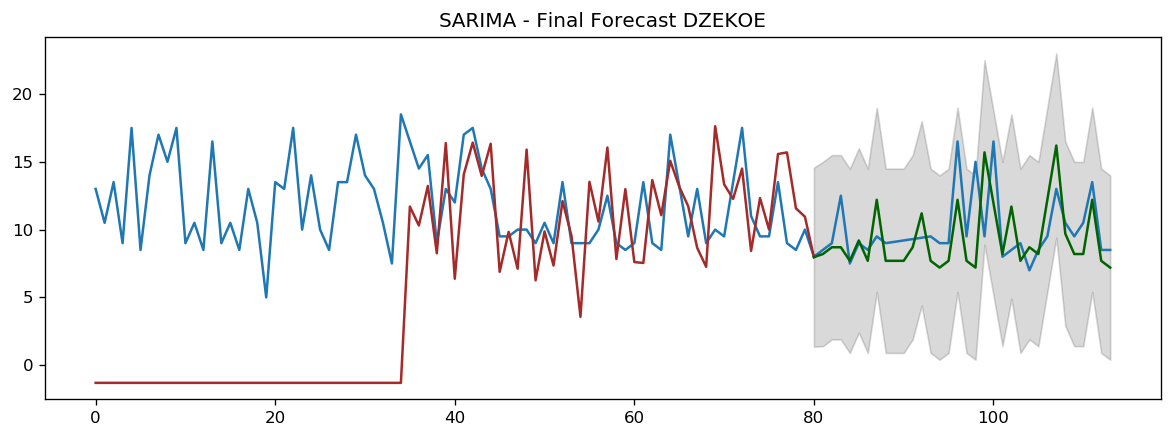
\includegraphics[scale=0.5]{images/dzeko_sarima_fantavoti.png}
   \caption{\textit{SARIMA forecast on ''Edin Dzeko''.}}
  \label{fig:sarima}
\end{figure}

\section{MLP}
The MLP model architecture includes 1 input layer with 12 nodes, 1 hidden layer with 38 nodes and 1 output layers with 1 node. The activation function is \textit{relu}.
The network has been trained with Adam optimizer and 150 epochs.
An example of application of the mlp model is visible in Figure \ref{fig:mlp}
\begin{figure}[H]
  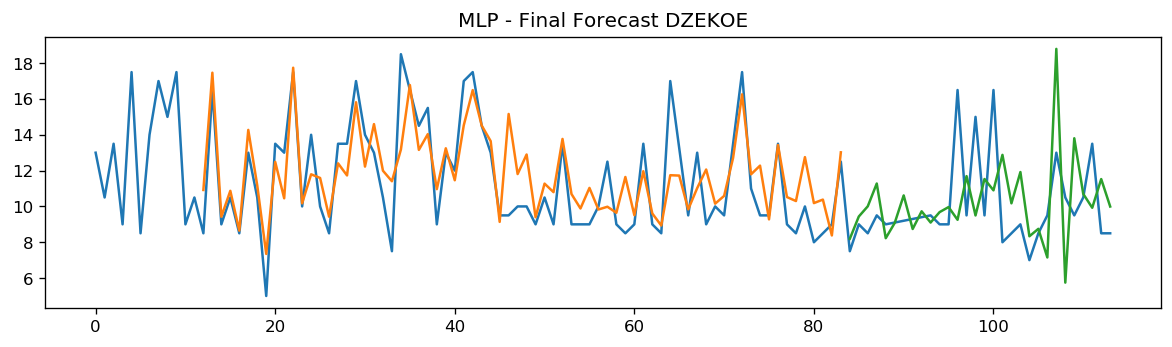
\includegraphics[scale=0.5]{images/dzeko_mlp_fantavoti.png}
   \caption{\textit{MLP forecast on ''Edin Dzeko''.}}
  \label{fig:mlp}
\end{figure}

\section{Models combination}

In order to improve accuracy (\textit{rmse}) on predictions, the two models were ensembled to come up with an hybrid version.
The final model used for forecasting is defined as:
\\
\begin{center}
  $\alpha * MLP + (1 - \alpha) * SARIMA$
\end{center}
where:
\begin{itemize}
    \item \textbf{$\alpha$} is a costant weight between 0 and 1 and is the value that minimizes the RMSE
    \item \textbf{MLP} is the value predicted by MLP model
    \item \textbf{SARIMA}  is the value predicted by SARIMA model 
\end{itemize}


\begin{figure}[H]
  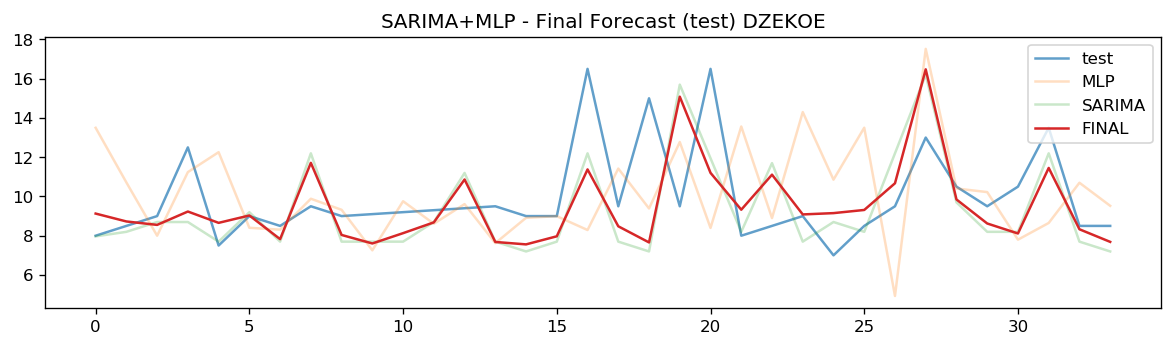
\includegraphics[scale=0.5]{images/dzeko_final_forecast.png}
   \caption{\textit{Final forecast on test set of ''Edin Dzeko''. $\alpha  = 0.21$, \textit{linear interpolation}}}
  \label{fig:mlp}
\end{figure}

\begin{figure}[H]
  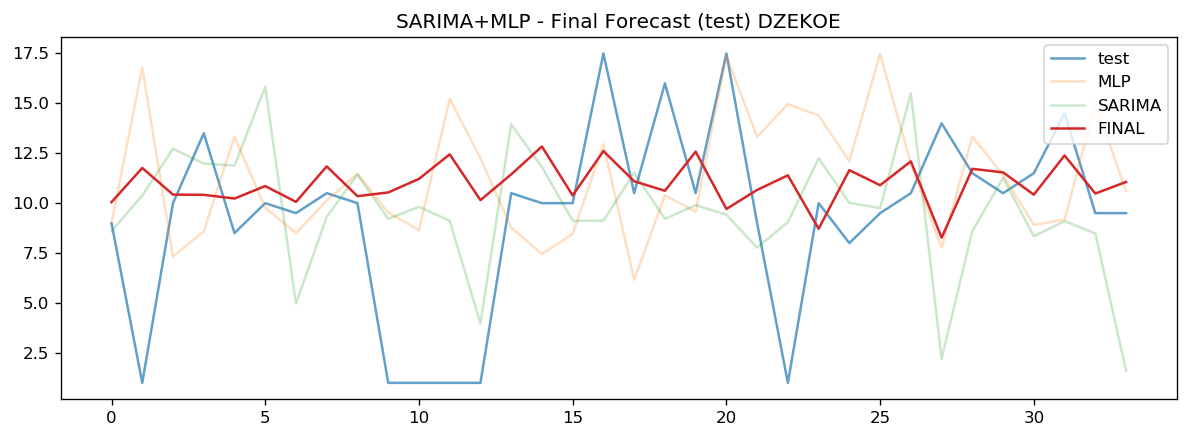
\includegraphics[scale=0.5]{images/dzeko_final_forecast_placeholder.png}
   \caption{\textit{Final forecast on test set of ''Edin Dzeko''. $\alpha  = 0.21$, \textit{placeholder}}}
  \label{fig:mlp}
\end{figure}



\begin{table}
 \begin{tabular}{|c|c|c|c|} 
 \hline
 Filling method & SARIMA+MLP & SARIMA & MLP \\
 \hline \hline
 Linear interpolation & 1.94 & 1.97 & 2.21 \\
 Placeholder & 3.48 & 4.22 & 4.31 \\
 \hline
 \end{tabular}
 \caption{\textit{Comparison between different models and filling methods using RMSE.}}
 \label{table:RMSE}
\end{table}








